\section{Problem Context}
\subsection{UK Statistics}
In the UK alone, around 2,000,000 people live with sight loss --- around 360,000 of which are registered with their local authority as being blind or visually impaired, who have severe and irreversible sight loss~/cite{uk-blind}.  Of these 360,000 people, there are only 17,000 white cane-users, and less than 4,800~\cite{guidedog-count} guide-dog owners. Assuming no overlap between guide dog users and white cane users, this leaves almost 94\% without access to the two major forms of assistance available to the blind.

A possible factor that could explain the relatively small adoption of Guide Dogs is their cost --- as mentioned in the introductory section, the life-time cost of a guide dog is around £50,000. Although the dog is paid for in it's entirety by the Guide Dogs for the Blind association, they themselves are a charity and do not receive government funding. A system whereby the visually impaired could purchase a guide-dog would likely not be effective, as 66\% of the registered blind/partially sighted are not in paid employment~\cite{afbff} so would be unlikely to be able to afford the cost.

\subsection{Developing Countries}
The situation in less developed countries than the UK is far worse. According to the Himalayan Cataract Project~\cite{worldblindness}, ``blindness is most prevalent in developing countries where malnutrition, inadequate health and education services, poor water quality and a lack of sanitation leads to a high incidence of eye disease''. If these countries are so impoverished that they are unable to afford services that are considered basic human rights in the developed world, it is unlikely that they will be able to afford to spend £50,000 per person on guide dogs. 

Although white canes are a cheaper, they are not without their downsides. They have limited range - typically a few feet in-front of the user. This makes finding doorways etc a more difficult task than when using a guide-dog. 

\section{The Problem}
This project aims to address the lack of a cheap, intuitive way of enhancing the mobility of the visually impaired.

It is non-trivial to convey visual information in the form of audio, for a number of reasons.

\subsection{Compression}
\label{sec:compression}
Measuring the bit-rate of sensory systems is not an easy task --- however, research has been done into the informational capacity of both the human visual system, and human auditory system.

Evidence makes it clear that the human visual system has a higher bit-rate than the human auditory system. Estimates by H. Jacobson~\cite{jacobson1950informational} suggest the informational capacity for the human ear to be roughly $8\times10^3$ bits/sec. In a separate paper~\cite{jacobson1951informational} Jacobson also estimates the informational capacity of the human eye to be around $4.3\times10^6$ bits/sec --- roughly $\times500$ higher. 

Taking this into consideration, it is clear that a working solution to the problem that this project aims to solve will involve compression of the visual information. 

\section{Existing Solutions}
Several attempts to solve the problem of video to audio conversion have been made in the past.

\subsection{vOICe}
The technique described as "An Experimental System for Auditory Image Representations"~\cite{vOICe} sonifies an object/scene by producing a 1:1 mapping from image to audio. This is accomplished by generating a sound, such that a visualisation of the frequency spectrum of the sound produces the input image. This technique has been used by the artist Aphex Twin in the song $\Delta M_i^{-1} = - \alpha \sum_{n=1}^N D_i \left[ n \right] \left[ \sum_{j \in C \left[ i \right]}^{} F_{ji} \left[ n -1 \right] + Fext_i \left[ n^{-1} \right] \right]$~\cite{aphex-equation} (more commonly known as [equation]), where viewing the song in a spectrogram produces a picture of the artists face:

\begin{figure}[H]
    \centering
    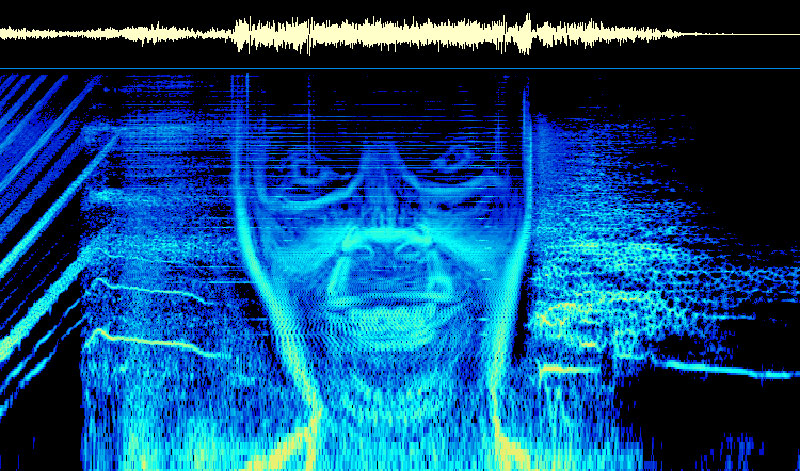
\includegraphics[width=\textwidth]{Background/equation-face.jpg}
    \caption{Spectrogram of $\Delta M_i^{-1} = - \alpha \sum_{n=1}^N D_i \left[ n \right] \left[ \sum_{j \in C \left[ i \right]}^{} F_{ji} \left[ n -1 \right] + Fext_i \left[ n^{-1} \right] \right]$~\cite{aphex-equation}}
\end{figure}

While this approach can theoretically convey all of the information held within the image, in practice, it is not feasible as a human visual aid. This method would require a human to perform a \ac{FFT} of the signal and re-construct the image in their head, and assumes that the auditory system has a sufficiently high bit-rate to receive all of the information, making the system unworkable --- little compression is performed. 

\subsection{Virtual Acoustic Space}
\label{sec:vas}
A paper by Gonzalez-Mora, J.L. et al~\cite{vas} describes a method involving \ac{VAS}. \ac{VAS} works by simulating the sound that a user would hear if a point source at a particular angle and distance from the user was emitting a tone. For each frame, several points are placed --- the field of view of the camera is divided into a $17\times9$ grid, with a point inserted in each division. 

The system is not totally dissimilar to echo-location, but uses a simulated response from the objects, rather than relying on an ultrasonic echo.

\begin{figure}[H]
    \centering
    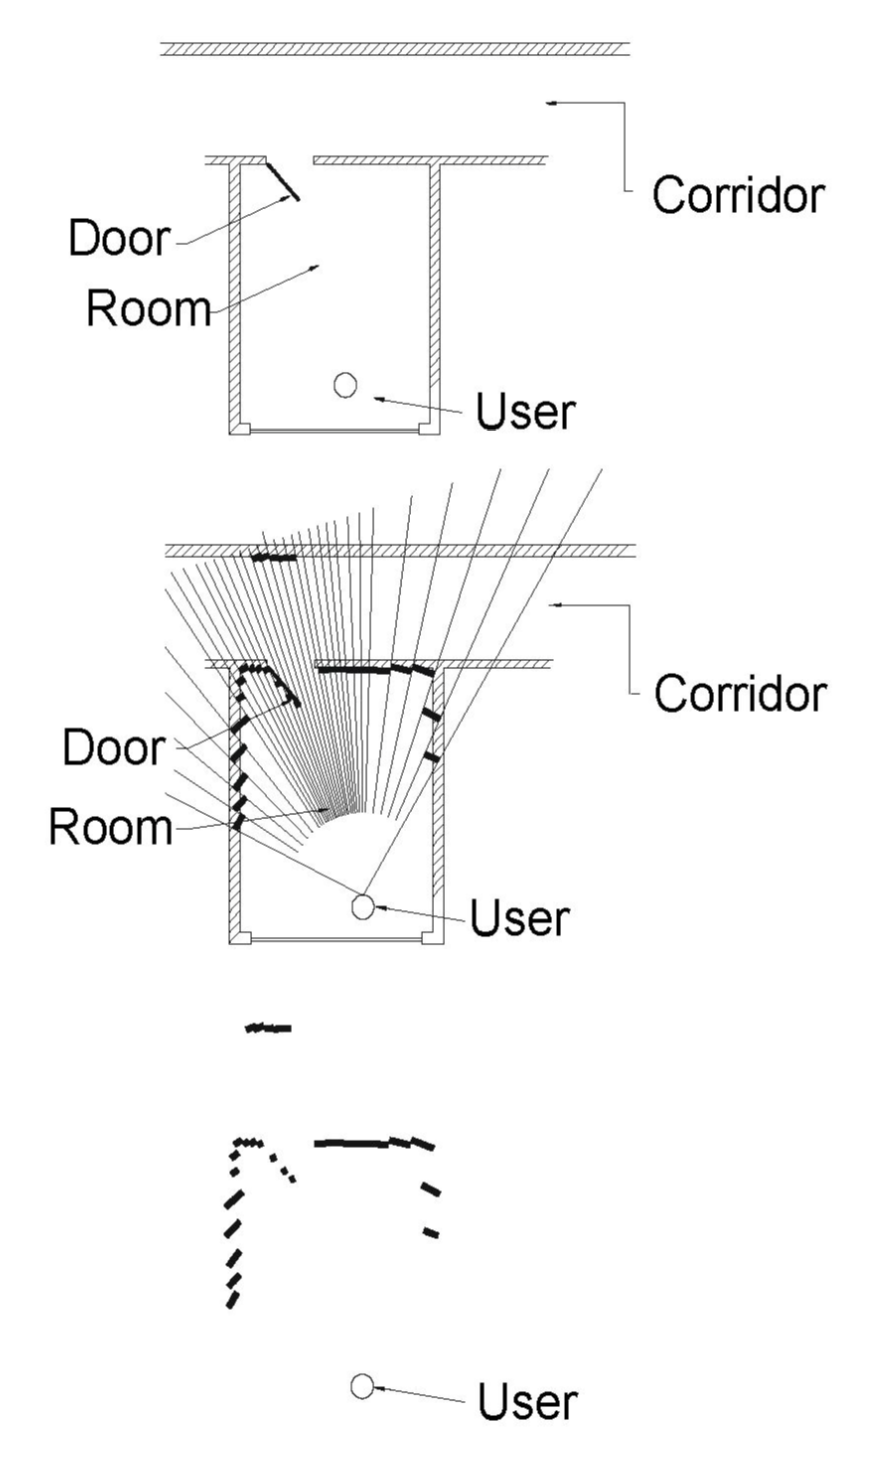
\includegraphics[width=0.5\textwidth]{Background/vas.png}
    \caption{Point placement with \ac{VAS}}
\end{figure}

The system described uses the \ac{HRTF} technique to apply filters to a tone. \ac{HRTF} works by modelling the effect the human body/head has on incoming audio. For instance, a tone emitted from a source to the left of a user has different properties when received on the left ear to the right ear; Higher frequencies will be attenuated more on the right ear, and there will be a slightly delay between the signal reaching each the right ear-drum compared to the left ear-drum. The \ac{HRTF} is applied to every point placed by the \ac{VAS} algorithm on both left and right channels. The modified tones (referred to as pips) are then played back in a random order. By inferring the position of each point based on it's acoustic properties, it has been shown that a trained user can navigate around a room.

\begin{figure}[H]
    \centering
    \includegraphics[width=0.25\textwidth]{Background/HRTF.png}
    \caption{Basis of HRTF technique~\cite{hrtf-diagram}}
\end{figure}

Although this system seems fairly effective, it is not without limitations.  

\subsection{TheVIBE}
``TheVIBE'' is a visuo-auditory sensory substitution system~\cite{thevibe}, which is similar in ways to the method discussed in section \ref{sec:vas}.

\begin{figure}[H]
    \centering
    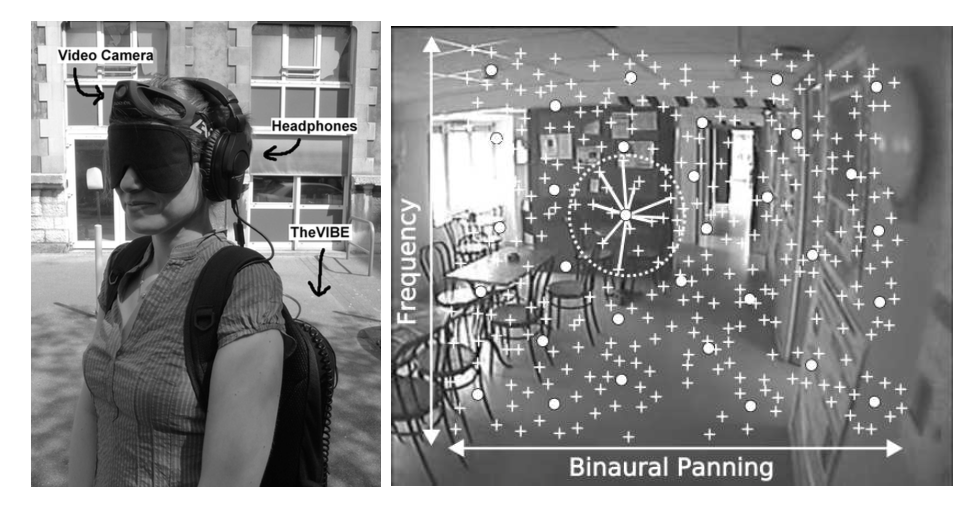
\includegraphics[width=0.5\textwidth]{Background/thevibe.png}
    \caption{Visualisation of point spacing in TheVIBE}
\end{figure}

This paper describes a technique whereby points are assigned to ``receptive fields''. Each field has a static position, and is assigned loudness, determined by the Z-axis position of the points within the field. Unlike the method discussed in section \ref{sec:vas}, TheVIBE does not use a full \ac{HRTF} to convey field position; rather, it uses an inter-aural loudness difference (similar to stereo panning) to describe horizontal position, and tone frequency variation to describe vertical position.

\section{Methods and Tools}
\subsection{Hardware}
The use of a depth-sensing camera has multiple advantages in the context of this project.

For navigational assistance, it is crucial to be able to know how far away obstacle are, so we are able to warn them that something is blocking their path.

It is also important when conveying the shape or structure of an object to a user. To extract an individual object from an image, we need to know the object boundaries. In a high contrast scenario --- for instance, a red object on a yellow background, this is possible using only image data. However, in a lower-contrast situation, for instance a gray object on a black background, this can be more difficult. This report details a method that allows depth information to be combined with image data, demonstrating improvements over image/depth segmentation alone. 

\subsection{Structured Light}
The XTION~\cite{xtion} device used in this project uses a technique involving structured light in order to compute the depth-map of a scene.

The XTION projects a known pattern of structured \ac{IR} laser light onto the scene, and using an \ac{IR} camera, receives the location and shape of each \ac{IR} point. The camera does not use a lens like those found on normal, visible-light cameras --- it has what's known as an astigmatic lens. An astigmatic lens has a focal-length along the X-axis that differs to that along the Y-axis. For instance, if the projected pattern consisted of many circular points, due to astigmatism in the lens, the image read back by the infra-red camera would consist of many elliptical points, varying in eccentricity according to distance between the point and the projector.

Using the change in eccentricity for each point, the device is able to construct a depth-map of the scene in real-time.

This sensor was developed by a company called Primesense, and is quite well supported --- drivers are available for all major platforms. The XTION is also supported by OpenNI, a framework used to develop software for ``Natural Interaction'' devices. 

\subsection{Other Techniques}
Use of structured light is not the old technique that has been developed to acquire depth-maps - other methods exist, for instance, Time-of-Flight and Stereoscopic systems. The Asus XTION was chosen over other devices, as it is fairly in-expensive (\~£100), and can be powered by USB alone (other devices, such as the Microsoft Kinect, require mains power to operate). 

\subsection{Software}
A majority of the development work done over the course of this project has been in Matlab, although Java and C++ have also been used.

\subsubsection{Matlab}
It was decided that Matlab was the right tool for the job for several reasons.

Firstly, Matlab has a lot of relevant functionality ``baked-in'' - for instance, an \ac{FFT} can be performed on a vector in one line: \lstinline$fft(vector)$, with no additional libraries required. This is not the case with many other languages. This makes prototyping much quicker, as it is not necessary to totally re-invent the wheel when trying new ideas.

Wrappers for OpenNI are available for Matlab, making interaction with the XTION camera - the wrapper is open-source, so any modifications can be made quite easily.

Another major factor in choosing Matlab over another language is the amount of support available, both physically from my Project Supervisor, and online from the Matlab community. 

The project has been developed using Matlab r2014a, although should be backwards-compatible with most recent releases. 

\subsubsection{Java}
As large parts of Matlab run in the \ac{JVM}, it is possible to use Java classes directly from within Matlab. This was taken advantage of in order to use threads, which is something that Matlab does not support out of the box. 

Matlab r2014a runs under the Java JVM version 1.7 - as such, any development must be done using the Java 7 JDK or below. 

\subsubsection{C/C++}
C/C++ functions can be exported to the Matlab environment through the use of MEX-files. The OpenNI wrapper used to interact with the XTION camera was written using C++ and MEX, and required some modifications.

Additionally, a C++ based Video Segmentation~\cite{videosegment} tool written by Google and Georgia Tech was trialled, and was also slightly modified.
